% 96-42(96쪽) — 삼각형 ABC 와 $\angle\pt{A}$ 의 이등분선 AD(원문 「오른쪽 그림」). 스캔 화질이 낮아 TikZ 로 다시 그림.
% 라벨은 원문 것만: 꼭짓점 A·B·C·D, 길이 4·2, $\angle\pt{A}$ 가 이등분된 표시(원문의 점 두 개).
% 길이 표시의 점선 호는 원문 꼴. $\seg{AD}$ 의 길이(답)는 그림에서 읽히지 않게 적지 않는다.
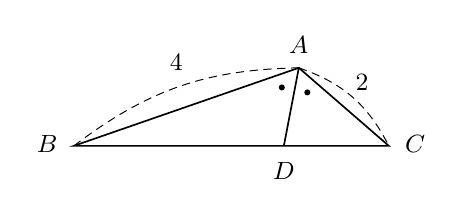
\begin{tikzpicture}[line width=0.6pt, x=1cm, y=1cm]
  \coordinate (B) at (0,0);
  \coordinate (C) at (4.0,0);
  \coordinate (A) at (2.857,0.991);
  \coordinate (D) at (2.667,0);
  \draw (A) -- (B) -- (C) -- cycle;
  \draw (A) -- (D);
  % 이등분된 두 각의 표시(원문의 점)
  \fill (2.641,0.742) circle (1.1pt);
  \fill (2.965,0.679) circle (1.1pt);
  % 길이 표시의 점선 호
  \draw[densely dashed, line width=0.35pt] (B) to[bend left=18] (A);
  \draw[densely dashed, line width=0.35pt] (A) to[bend left=22] (C);
  \node[font=\small] at (1.30,1.06) {$4$};
  \node[font=\small] at (3.66,0.80) {$2$};
  \node[font=\small, anchor=east] at (-0.08,0.02) {$\pt{B}$};
  \node[font=\small, anchor=west] at (4.08,0.02) {$\pt{C}$};
  \node[font=\small, anchor=south] at (2.857,1.04) {$\pt{A}$};
  \node[font=\small, anchor=north] at (2.667,-0.08) {$\pt{D}$};
\end{tikzpicture}
